% Options for packages loaded elsewhere
\PassOptionsToPackage{unicode}{hyperref}
\PassOptionsToPackage{hyphens}{url}
%
\documentclass[
]{article}
\usepackage{amsmath,amssymb}
\usepackage{iftex}
\ifPDFTeX
  \usepackage[T1]{fontenc}
  \usepackage[utf8]{inputenc}
  \usepackage{textcomp} % provide euro and other symbols
\else % if luatex or xetex
  \usepackage{unicode-math} % this also loads fontspec
  \defaultfontfeatures{Scale=MatchLowercase}
  \defaultfontfeatures[\rmfamily]{Ligatures=TeX,Scale=1}
\fi
\usepackage{lmodern}
\ifPDFTeX\else
  % xetex/luatex font selection
\fi
% Use upquote if available, for straight quotes in verbatim environments
\IfFileExists{upquote.sty}{\usepackage{upquote}}{}
\IfFileExists{microtype.sty}{% use microtype if available
  \usepackage[]{microtype}
  \UseMicrotypeSet[protrusion]{basicmath} % disable protrusion for tt fonts
}{}
\makeatletter
\@ifundefined{KOMAClassName}{% if non-KOMA class
  \IfFileExists{parskip.sty}{%
    \usepackage{parskip}
  }{% else
    \setlength{\parindent}{0pt}
    \setlength{\parskip}{6pt plus 2pt minus 1pt}}
}{% if KOMA class
  \KOMAoptions{parskip=half}}
\makeatother
\usepackage{xcolor}
\usepackage[margin=1in]{geometry}
\usepackage{longtable,booktabs,array}
\usepackage{calc} % for calculating minipage widths
% Correct order of tables after \paragraph or \subparagraph
\usepackage{etoolbox}
\makeatletter
\patchcmd\longtable{\par}{\if@noskipsec\mbox{}\fi\par}{}{}
\makeatother
% Allow footnotes in longtable head/foot
\IfFileExists{footnotehyper.sty}{\usepackage{footnotehyper}}{\usepackage{footnote}}
\makesavenoteenv{longtable}
\usepackage{graphicx}
\makeatletter
\def\maxwidth{\ifdim\Gin@nat@width>\linewidth\linewidth\else\Gin@nat@width\fi}
\def\maxheight{\ifdim\Gin@nat@height>\textheight\textheight\else\Gin@nat@height\fi}
\makeatother
% Scale images if necessary, so that they will not overflow the page
% margins by default, and it is still possible to overwrite the defaults
% using explicit options in \includegraphics[width, height, ...]{}
\setkeys{Gin}{width=\maxwidth,height=\maxheight,keepaspectratio}
% Set default figure placement to htbp
\makeatletter
\def\fps@figure{htbp}
\makeatother
\setlength{\emergencystretch}{3em} % prevent overfull lines
\providecommand{\tightlist}{%
  \setlength{\itemsep}{0pt}\setlength{\parskip}{0pt}}
\setcounter{secnumdepth}{5}
\usepackage{amsmath}
\ifLuaTeX
  \usepackage{selnolig}  % disable illegal ligatures
\fi
\usepackage{bookmark}
\IfFileExists{xurl.sty}{\usepackage{xurl}}{} % add URL line breaks if available
\urlstyle{same}
\hypersetup{
  pdftitle={Data Science 2 Midterm},
  pdfauthor={Jasmin Martinez (JRM2319), Ixtaccihuatl Obregon, Elliot Kim},
  hidelinks,
  pdfcreator={LaTeX via pandoc}}

\title{Data Science 2 Midterm}
\author{Jasmin Martinez (JRM2319), Ixtaccihuatl Obregon, Elliot Kim}
\date{03/24/2025}

\begin{document}
\maketitle

{
\setcounter{tocdepth}{2}
\tableofcontents
}
\section{Exploratory Analysis}\label{exploratory-analysis}

For datasets \textbf{dat1} and \textbf{dat2} initial exploration of the data structure, descriptive statistics of continuous variables, correlation analysis, and various visualization techniques were conducted.

Looking at \textbf{dat1}, the distribution of \textbf{log\_antibody} is approximately normal, as seen in Figure \ref{fig:d1-log-antibody-hist} and Figure \ref{fig:d1-log-antibody-qq}. High and low outliers can be observed in the Figure \ref{fig:d1-log-antibody-box}. Most covariates have weak or low correlation with each other. There is a high positive correlation between \textbf{bmi} and \textbf{weight} (\(\rho = 0.72\)) and a moderate negative correlation between \textbf{bmi} and \textbf{height} (\(\rho = -0.50\)). There is a mild negative correlation between \textbf{log\_antibody} and \textbf{bmi} (\(\rho = -0.23\)), \textbf{weight} (\(\rho = -0.17\)), and \textbf{age} (\(\rho = -0.15\)). There is a mild positive correlation between \textbf{log\_antibody} and \textbf{height} (\(\rho = 0.10\)). The correlation between \textbf{log\_antibody} and \textbf{SBP} (\(\rho = -0.06\)), \textbf{LDL} (\(\rho = -0.04\)), and \textbf{time} (\(\rho = -0.01\)) are near zero, indicating no linear relationship. Linear relationships can be seen in Figure \ref{fig:d1-log-antibody-lin}.

Exploring \textbf{dat2}, the distribution of \textbf{log\_antibody} is also approximately normal, as shown Figure \ref{fig:d2-log-antibody-hist} and Figure \ref{fig:d2-log-antibody-qq}. High and low outliers are again visible in the Figure \ref{fig:d2-log-antibody-box}. Most covariates exhibit weak or low correlation with each other. There is a high positive correlation between \textbf{bmi} and \textbf{weight} (\(\rho = 0.72\)) and a moderate negative correlation between \textbf{bmi} and \textbf{height} (\(\rho = -0.53\)). There is a mild negative correlation between \textbf{log\_antibody} and \textbf{bmi} (\(\rho = -0.16\)), \textbf{weight} (\(\rho = -0.11\)), and \textbf{age} (\(\rho = -0.08\)). A mild positive correlation exists between \textbf{log\_antibody} and \textbf{height} (\(\rho = 0.084\)). The correlations between \textbf{log\_antibody} and \textbf{SBP} (\(\rho = -0.01\)), \textbf{LDL} (\(\rho = -0.00\)), and \textbf{time} (\(\rho = -0.25\)) are near zero or weak, again suggesting no strong linear relationship. Linear relationships can be seen in Figure \ref{fig:d2-log-antibody-lin}.

The exploration and evaluation of \textbf{dat1} is used to help build a prediction model specific ally using GAM to understand how demographic and clinical factors influence antibody responses and how antibody levels change over time following vaccination. Considering the researcher collects a new and independent dataset, \textbf{dat2}, we discover the correlation between \textbf{time} and \textbf{log\_antibody} is stronger than in \textbf{dat1} and similarly has weak linear relationships with most covariates. \textbf{Dat2} allows us to evaluate the robustness and generalizability of our prediction model.

\section{Model Trainging}\label{model-trainging}

The \textbf{dat1} dataset is the designated training data and \textbf{dat2} is the testing dataset. Using the \textbf{train()} function, a multiple linear regression , ridge, lasso, generalized additive model, and a multivariate adaptive regression splines model were fitted to determine the optimal model for the data. All models used a 10-fold cross-validation that was determined by using \textbf{method = cv} and \textbf{number = 10} in the \textbf{trainControl()} function.

\textbf{Multiple Linear Regression Model}
A multiple linear regression model is simple and easy to use when working with linearly dependent data but works under the assumption of homoscedasticity and no multicollinearity. Fitting this model required \textbf{method = lm} in the \textbf{train()} function, resulting in \(R^2 = 0.1470498\) and \(R_{adj}^2 = 0.03320516\) indicating a poor fit.

\textbf{Ridge and Lasso Regression}

Ridge and lasso models are useful for improving prediction accuracy when dealing with multiple predictors. These models help prevent overfitting through the inclusion of a penalty term that regularizes coefficient estimates. A key component to these models is the lambda tuning parameter, which controls the strength of the penality applied to the coefficients.

The models were fit using the Caret train() function and specifying the method = ``glmnet'', which allows the adjustment of the alpha parameter in which alpha = 1 for a lasso regression (L1 regularization) and alpha = 0 for a ridge regression (L2 regularization). The tuning parameter (lambda) for each model was selected by a 10-fold cross-validation. To explore a wide range of lambda values, a sequence of 100 exponentially spaced values between -5 and 6 was specified in the tuneGrid argument of Caret's train() function. These models assume that the relationship between the predictors and the outcome is linear.

While the lasso regression model conducts variable selection by shrinking coefficients to 0, the ridge regression model can only shrink coefficients towards 0. Therefore, the lasso regression model is useful for handling multiple predictors while the ridge regression model helps reduce the size of the coefficients for all predictors and is useful for handling predictors that are highly correlated, thereby preventing multicollinearity.

\textbf{Generalized Additive Model (GAM)}

A Generalized Additive Model (GAM) was created to model log-transformed antibody level. Predictors included age, gender, race, smoking, height, weight, BMI, diabetes, hypertension, SBP, LDL, and time since vaccination. To prepare the data for modeling, the model matrix, x, was created using the outcome and all predictors listed above and extracted the response variable, y. Given that race and smoking were categorical variables with multiple categories, some re-coding was necessary to use these variables in the model building. Therefore, race and smoking were converted into factor variables with ``White'' being the reference group for race and ``Never'' being the reference group for smoking.

The GAM models were then fitted. The first model, gam.m1, is a standard linear model with no smoothing terms. The second model, gam.m2, uses smoothing on age, bmi, SBP, LDL, and time since vaccination. There was reason to believe these variables were non-linear, therefore the smoothing allowed the variables to be used in the model. Finally, model 3, gam.m3, includes a tensor product to model the interaction between height and weight.

The three GAM models were then compared using an ANOVA test that provides the f-test; this was used to determine which model provides the best fit. Cross-validation for GAM tuning was then conducted using a 10-fold cross-validation to tune to GAM model. The best hyperparameters and the final fitted model were then retrieved. The same model training procedure was used with the new, independent dataset, dat2.

Model 2 (gam.m2) was chosen to be the final model based on the improvements it made upon Model 1 (gam.m1), (pval=\textless0.001).

\textbf{Multivariate Adaptive Regression Splines Model}

The Multivariate Adaptive Regression Splines (MARS) model is a flexible non-linear model technique used to evaluate the relationship between an outcome and multiple covariates. MARS divides the data into segments and fits a piecewise linear regressions for each segment. MARS is used to model \textbf{log\_antibody} levels based on clinical and demographic predictors. The model is tuned on two hyperparameters: \textbf{nprune} for the most number of terms and \textbf{degree} for the most amount of degree interactions between predictors.

\textbf{Re-sampling and final model selection}

We used the \textbf{resample()} function to conduct a robust comparison of all the models listed above, with the performance metric being the Root Mean Squared Error (RMSE). The models included in this analysis were Multiple Linear Regression, Lasso Regression, Ridge Regression, Multivariate Adaptive Regression Splines (MARS), and the Generalized Additive Model (GAM). As illustrated in the results below, the GAM model demonstrated the lowest RMSE, with a value of 0.531, indicating its superior predictive accuracy. This was closely followed by the MARS model, which had an RMSE of 0.530, highlighting its strong performance as well. Consistent with expectations, the simplest model, Multiple Linear Regression, exhibited the highest RMSE of 0.552, reflecting its limitations in capturing complex relationships within the data compared to more advanced models.

\section{Final Model Results}\label{final-model-results}

The final model to predict \textbf{log\_antibody} levels was the Generalized Additive (GAM) Model. The model equation is given by:
\[
\begin{aligned}
\text{log_antibody}_i =\ & 
\mathbf{10.23} 
- \mathbf{0.30} \cdot \text{gender}_i 
+ \mathbf{0.014} \cdot \text{diabetes}_i 
- \mathbf{0.0078} \cdot \text{hypertension}_i \\
& + \mathbf{0.0222} \cdot \text{smokingFormer}_i 
- \mathbf{0.1932} \cdot \text{smokingCurrent}_i \\
& - \mathbf{0.0033} \cdot \text{raceAsian}_i 
- \mathbf{0.0105} \cdot \text{raceBlack}_i 
- \mathbf{0.0374} \cdot \text{raceHispanic}_i \\
& + f_1(\text{age}_i) 
+ f_2(\text{SBP}_i) 
+ f_3(\text{LDL}_i) 
+ f_4(\text{bmi}_i) \\
& + f_5(\text{time}_i) 
+ f_6(\text{height}_i) 
+ f_7(\text{weight}_i) 
+ \varepsilon_i
\end{aligned}
\]

Using GAM allows for flexibility and interpretability for non-linear relationships. After comparing GAM specification via ANOVA for model 1, model2, and model 3 for \textbf{dat1} and \textbf{dat2}, model 2 was chosen. The model has an adjusted \(R^2 = 0.22\), showing non-linear effects contribute meaningful variance explanation. Some significant predictors would be gender, smoking, smmoth(age), amoth(bmi), and smooth(time), all with pval\textless0.0.001)

The prediction model's robustness and generalizability is mostly acceptable for \textbf{dat2}. Prediction accuracy was determined by the mean squared error (MSE) at 0.325 showing a low average on unseen data. The prediction model shows model stability with generalized cross-validation (GCV) score of 0.279. Looking at \ref{fig:dx-plots} we evaluate Predicted vs Actual log\_antibody Levels, Residuals vs Predicted, and the Distribution of Residuals. Predictions are mostly aligned with the observed values especially in the 9.5-10.5 predicted range. There is mild under-prediction below value 9, which indicates that the model may tend to underestimate lower antibody levels but perform well in the 9.5-10.5 predicted range. The predicted vs residual plot shows residuals mostly centered and near 0. Right-skewness can be observed in the predicted vs residual plots, which could suggest some non-linearity. The distribution of residuals looks approximately normal and does not have extreme outliers or multi-modality.

\newpage

\begin{table}

\caption{\label{tab:unnamed-chunk-4}Clean Summary Statistics for Numeric Variables}
\centering
\begin{tabular}[t]{l|r|r|r|r|r|r}
\hline
Variable & Min & Q1 & Median & Mean & Q3 & Max\\
\hline
id & 1.000000 & 1250.750000 & 2500.50000 & 2500.50000 & 3750.25000 & 5000.00000\\
\hline
age & 44.000000 & 57.000000 & 60.00000 & 59.96840 & 63.00000 & 75.00000\\
\hline
gender & 0.000000 & 0.000000 & 0.00000 & 0.48540 & 1.00000 & 1.00000\\
\hline
height & 150.200000 & 166.100000 & 170.10000 & 170.12634 & 174.22500 & 192.90000\\
\hline
weight & 56.700000 & 75.400000 & 80.10000 & 80.10908 & 84.90000 & 106.00000\\
\hline
bmi & 18.200000 & 25.800000 & 27.60000 & 27.74040 & 29.50000 & 38.80000\\
\hline
diabetes & 0.000000 & 0.000000 & 0.00000 & 0.15440 & 0.00000 & 1.00000\\
\hline
hypertension & 0.000000 & 0.000000 & 0.00000 & 0.45960 & 1.00000 & 1.00000\\
\hline
SBP & 101.000000 & 124.000000 & 130.00000 & 129.90040 & 135.00000 & 155.00000\\
\hline
LDL & 43.000000 & 96.000000 & 110.00000 & 109.90860 & 124.00000 & 185.00000\\
\hline
time & 30.000000 & 76.000000 & 106.00000 & 108.86260 & 138.00000 & 270.00000\\
\hline
log & 7.765405 & 9.681635 & 10.08908 & 10.06434 & 10.47758 & 11.96137\\
\hline
\end{tabular}
\end{table}

\begin{figure}

{\centering 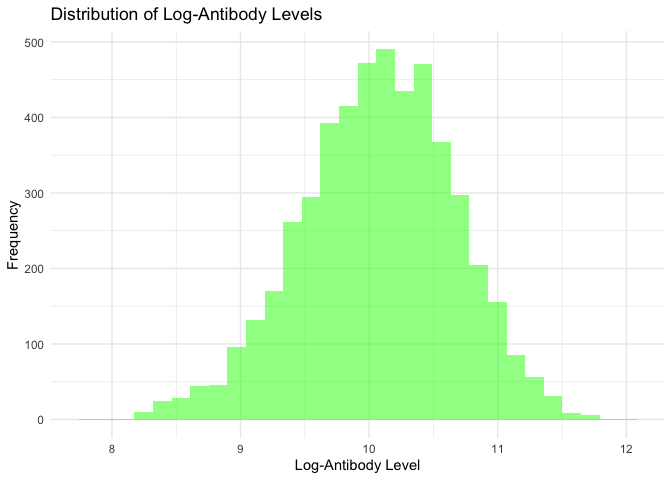
\includegraphics[width=0.33\linewidth]{DS2_Midterm_files/figure-latex/d1-log-antibody-hist-1} 

}

\caption{Histogram of log\_antibody levels for dat1}\label{fig:d1-log-antibody-hist}
\end{figure}

\begin{figure}

{\centering 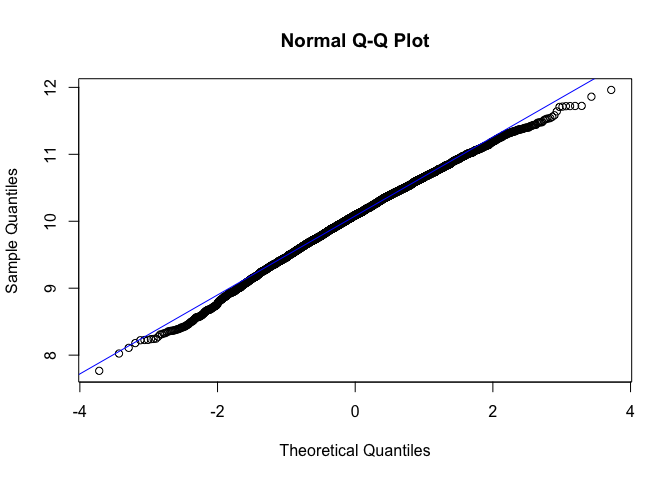
\includegraphics[width=0.33\linewidth]{DS2_Midterm_files/figure-latex/d1-log-antibody-qq-1} 

}

\caption{Q-Q plot of log\_antibody levels for dat1}\label{fig:d1-log-antibody-qq}
\end{figure}

\begin{figure}

{\centering 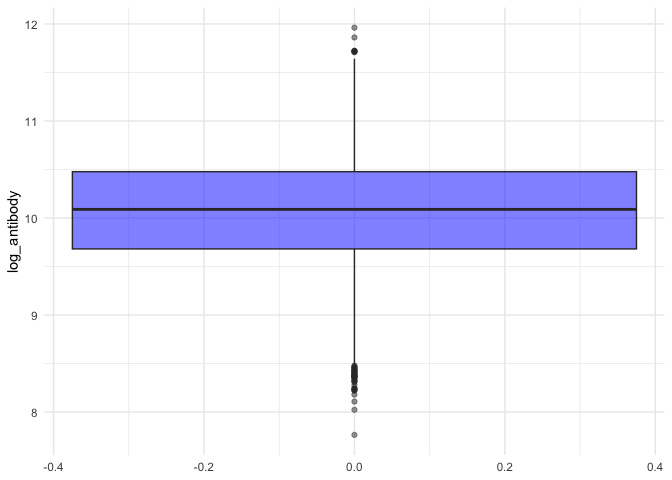
\includegraphics[width=0.33\linewidth]{DS2_Midterm_files/figure-latex/d1-log-antibody-box-1} 

}

\caption{Boxplot of log\_antibody levels for dat1}\label{fig:d1-log-antibody-box}
\end{figure}

\begin{figure}
\centering
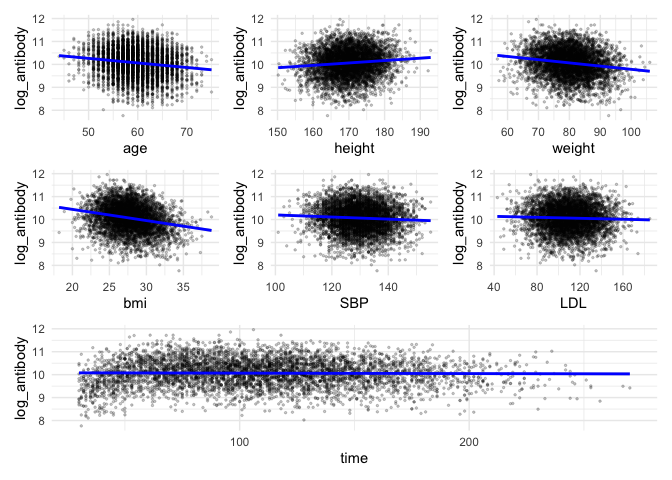
\includegraphics{DS2_Midterm_files/figure-latex/d1-log-antibody-lin-1.pdf}
\caption{\label{fig:d1-log-antibody-lin}Linearity between log\_antibody levels and covariates for dat1}
\end{figure}

\begin{figure}

{\centering 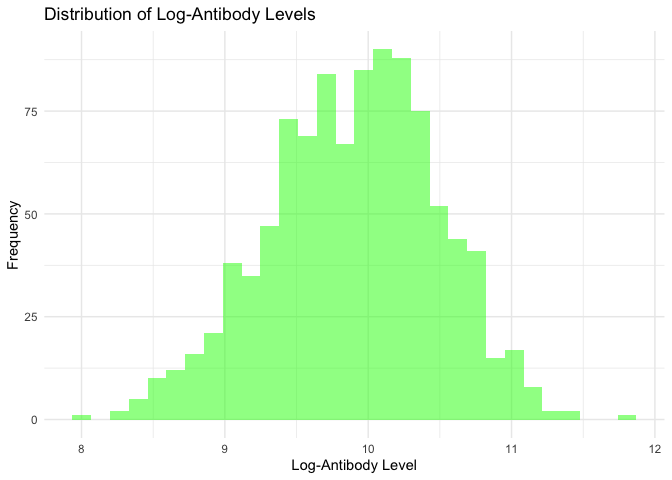
\includegraphics[width=0.33\linewidth]{DS2_Midterm_files/figure-latex/d2-log-antibody-hist-1} 

}

\caption{Histogram of log\_antibody levels for dat2}\label{fig:d2-log-antibody-hist}
\end{figure}

\begin{figure}

{\centering 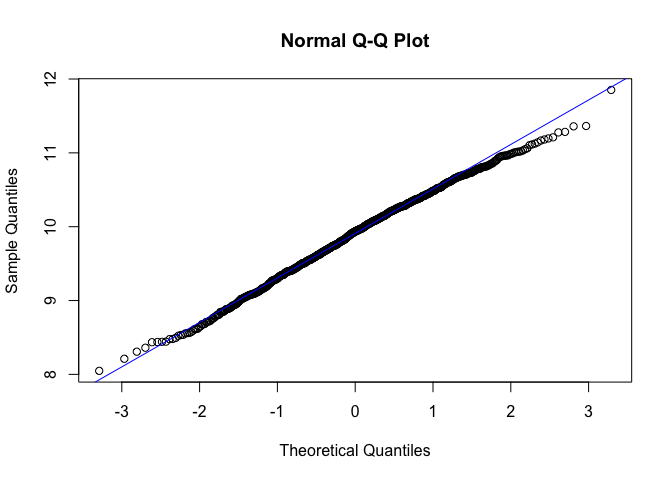
\includegraphics[width=0.33\linewidth]{DS2_Midterm_files/figure-latex/d2-log-antibody-qq-1} 

}

\caption{Q-Q plot of log\_antibody levels for dat2}\label{fig:d2-log-antibody-qq}
\end{figure}

\begin{figure}

{\centering 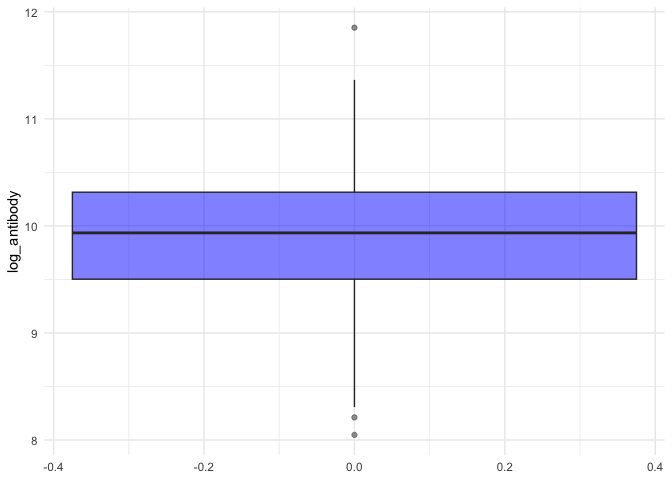
\includegraphics[width=0.33\linewidth]{DS2_Midterm_files/figure-latex/d2-log-antibody-box-1} 

}

\caption{Boxplot of log\_antibody levels for dat2}\label{fig:d2-log-antibody-box}
\end{figure}

\begin{figure}
\centering
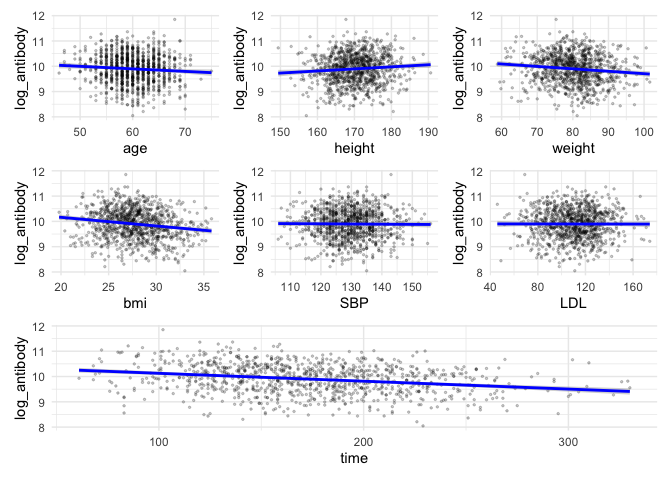
\includegraphics{DS2_Midterm_files/figure-latex/d2-log-antibody-lin-1.pdf}
\caption{\label{fig:d2-log-antibody-lin}Linearity between log\_antibody levels and covariates for dat2}
\end{figure}

\includegraphics{DS2_Midterm_files/figure-latex/unnamed-chunk-17-1.pdf}

\begin{verbatim}
## Warning in nominalTrainWorkflow(x = x, y = y, wts = weights, info = trainInfo, : There were missing values in resampled performance measures.
\end{verbatim}

\includegraphics{DS2_Midterm_files/figure-latex/unnamed-chunk-17-2.pdf}

\begin{verbatim}
##   alpha     lambda
## 7     0 0.01312373
\end{verbatim}

\begin{verbatim}
## 17 x 1 sparse Matrix of class "dgCMatrix"
##                           s1
## (Intercept)     1.274791e+01
## id             -1.894551e-06
## age            -1.977970e-02
## gender         -2.880556e-01
## raceAsian      -4.051537e-03
## raceBlack      -6.683819e-03
## raceHispanic   -4.179393e-02
## smokingFormer   2.418667e-02
## smokingCurrent -1.847083e-01
## height         -2.046729e-04
## weight         -9.107320e-04
## bmi            -4.735061e-02
## diabetes        1.128129e-02
## hypertension   -1.636703e-02
## SBP             1.066327e-03
## LDL            -1.608202e-04
## time           -2.795454e-04
\end{verbatim}

\begin{verbatim}
## Warning in nominalTrainWorkflow(x = x, y = y, wts = weights, info = trainInfo, : There were missing values in resampled performance measures.
\end{verbatim}

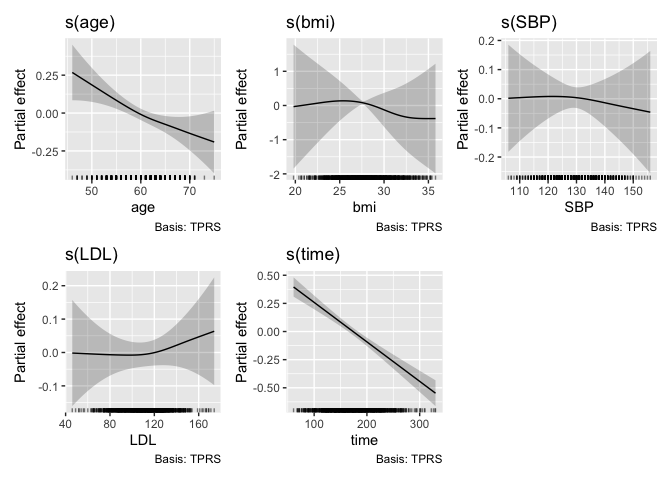
\includegraphics{DS2_Midterm_files/figure-latex/unnamed-chunk-18-1.pdf}

\begin{table}

\caption{\label{tab:tune-table}Optimal Tuning Parameters for Ridge and Lasso Regression}
\centering
\begin{tabular}[t]{l|r|r}
\hline
Model & Alpha & Lambda\\
\hline
Ridge & 0 & 0.0131237\\
\hline
Lasso & 1 & 0.0075298\\
\hline
\end{tabular}
\end{table}

\begin{table}

\caption{\label{tab:d1-anova-table}ANOVA Comparison of GAM Models (Dat1)}
\centering
\begin{tabular}[t]{l|r|r|r|r|r|r}
\hline
Model & Resid. Df & Resid. Dev & Df & Deviance & F & Pr(>F)\\
\hline
gam.m1 & 4984.000 & 1509.442 & NA & NA & NA & NA\\
\hline
gam.m2 & 4971.177 & 1380.053 & 12.82350 & 129.389611 & 36.37749 & 0.0000000\\
\hline
gam.m3 & 4968.540 & 1378.818 & 2.63652 & 1.234568 & 1.68820 & 0.1738572\\
\hline
\end{tabular}
\end{table}

\begin{figure}
\centering
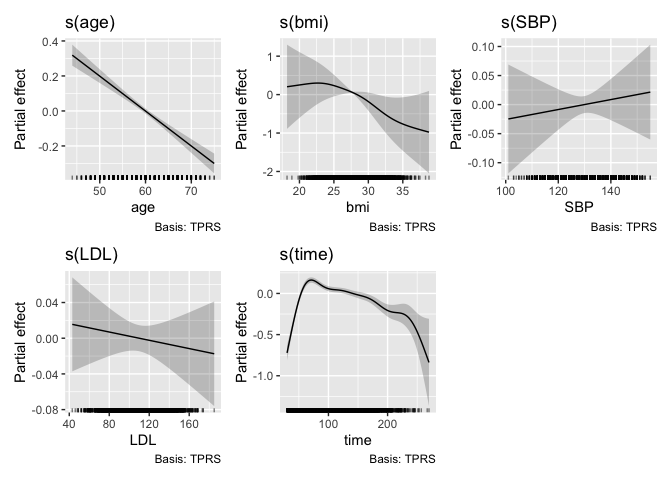
\includegraphics{DS2_Midterm_files/figure-latex/gam2-gridplot-1.pdf}
\caption{\label{fig:gam2-gridplot}Smooth terms for GAM model (gam.m2)}
\end{figure}

\begin{table}

\caption{\label{tab:d2-anova-table}ANOVA Comparison of GAM Models (Dat2)}
\centering
\begin{tabular}[t]{l|r|r|r|r|r|r}
\hline
Model & Resid. Df & Resid. Dev & Df & Deviance & F & Pr(>F)\\
\hline
gam.m1 & 984.0000 & 275.4546 & NA & NA & NA & NA\\
\hline
gam.m2 & 977.7820 & 268.5783 & 6.217997 & 6.8762407 & 4.0341782 & 0.0004416\\
\hline
gam.m3 & 976.6323 & 268.2745 & 1.149679 & 0.3038207 & 0.9640406 & 0.3384056\\
\hline
\end{tabular}
\end{table}

\includegraphics{DS2_Midterm_files/figure-latex/unnamed-chunk-21-1.pdf}

\begin{verbatim}
## 
## Family: gaussian 
## Link function: identity 
## 
## Formula:
## .outcome ~ gender + diabetes + hypertension + smoking + race + 
##     s(age) + s(SBP) + s(LDL) + s(bmi) + s(time) + s(height) + 
##     s(weight)
## 
## Parametric coefficients:
##                 Estimate Std. Error t value Pr(>|t|)    
## (Intercept)    10.228177   0.015328 667.269  < 2e-16 ***
## gender         -0.297837   0.014933 -19.945  < 2e-16 ***
## diabetes        0.014230   0.020640   0.689    0.491    
## hypertension   -0.007678   0.015995  -0.480    0.631    
## smokingFormer   0.022219   0.016660   1.334    0.182    
## smokingCurrent -0.193175   0.025834  -7.478  8.9e-14 ***
## raceAsian      -0.003296   0.033009  -0.100    0.920    
## raceBlack      -0.010509   0.018837  -0.558    0.577    
## raceHispanic   -0.037424   0.026176  -1.430    0.153    
## ---
## Signif. codes:  0 '***' 0.001 '**' 0.01 '*' 0.05 '.' 0.1 ' ' 1
## 
## Approximate significance of smooth terms:
##                 edf Ref.df      F p-value    
## s(age)    9.908e-01      9 13.733  <2e-16 ***
## s(SBP)    6.175e-07      9  0.000   0.765    
## s(LDL)    6.648e-07      9  0.000   0.639    
## s(bmi)    4.179e+00      9 41.897  <2e-16 ***
## s(time)   7.892e+00      9 44.960  <2e-16 ***
## s(height) 1.234e+00      9  0.278   0.121    
## s(weight) 2.262e-06      9  0.000   0.666    
## ---
## Signif. codes:  0 '***' 0.001 '**' 0.01 '*' 0.05 '.' 0.1 ' ' 1
## 
## R-sq.(adj) =   0.22   Deviance explained = 22.4%
## GCV = 0.27867  Scale est. = 0.27738   n = 5000
\end{verbatim}

\begin{figure}
\centering
\includegraphics{DS2_Midterm_files/figure-latex/mars-plots-1.pdf}
\caption{\label{fig:mars-plots}MARS Tuning Grid Selection}
\end{figure}

\begin{figure}
\centering
\includegraphics{DS2_Midterm_files/figure-latex/rs-plots-1.pdf}
\caption{\label{fig:rs-plots}Model Comparison (RMSE)}
\end{figure}

\begin{figure}
\centering
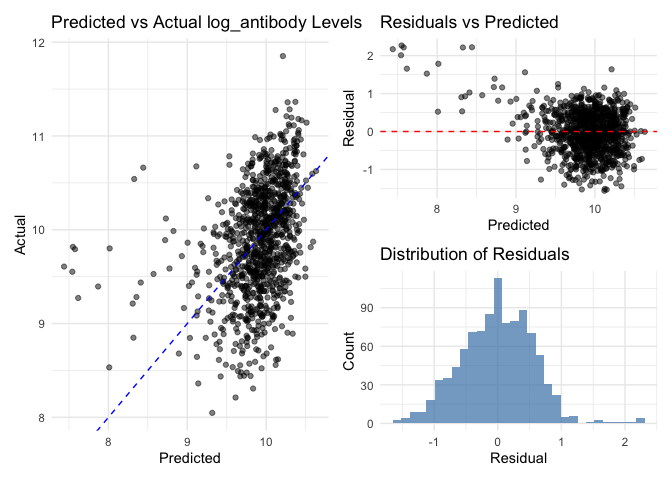
\includegraphics{DS2_Midterm_files/figure-latex/dx-plots-1.pdf}
\caption{\label{fig:dx-plots}Diagnostic Plots for Prediction Model on dat2}
\end{figure}

\end{document}
